\documentclass{article}%
\usepackage[T1]{fontenc}%
\usepackage[utf8]{inputenc}%
\usepackage{lmodern}%
\usepackage{textcomp}%
\usepackage{lastpage}%
\usepackage[head=40pt,margin=0.5in,bottom=0.6in]{geometry}%
\usepackage{graphicx}%
%
\title{\textbf{Madre venezolana: Estoy muy contenta porque en el buque operaron a mi hija}}%
\author{El Nacional Web | Con información de Fabiana Cantos | Enviada Especial}%
\date{27/11/2018}%
%
\begin{document}%
\normalsize%
\maketitle%
\textbf{URL: }%
http://www.el{-}nacional.com/noticias/sociedad/madre{-}venezolana{-}estoy{-}muy{-}contenta{-}porque{-}buque{-}operaron{-}hija\_261317\newline%
%
\textbf{Periodico: }%
EN, %
ID: %
261317, %
Seccion: %
Sociedad\newline%
%
\textbf{Palabras Claves: }%
Latinoamérica, Colombia, Sociedad\newline%
%
\textbf{Derecho: }%
2.1, %
Otros Derechos: %
, %
Sub Derechos: %
2.1.1\newline%
%
\textbf{EP: }%
NO\newline%
\newline%
%
\textbf{\textit{El doctor Rafael Gottenger, quien ofrece sus servicios en la actual misión del buque hospital Comfort USNS, destacó que la operaciópn que requería la menor tiene un monto aproximado de 2.000 y 3.000 dólares~}}%
\newline%
\newline%
%
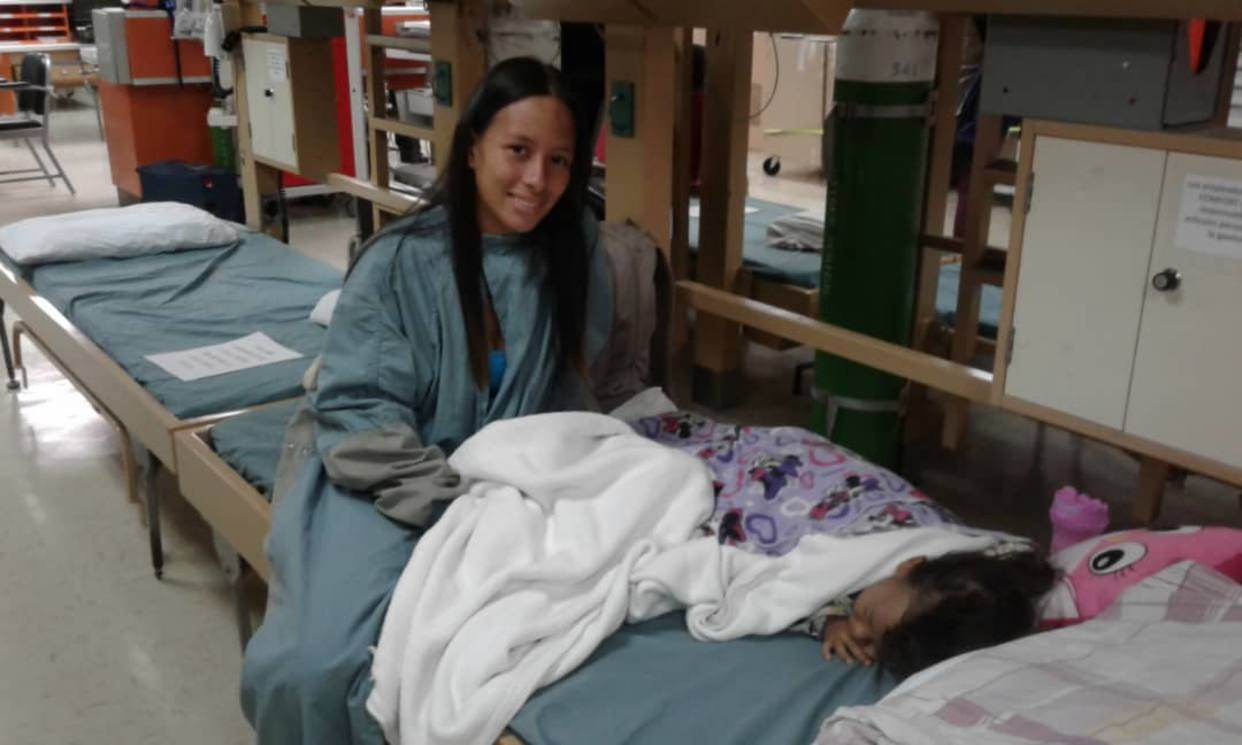
\includegraphics[width=300px]{25.jpg}%
\newline%
%
Rubilet Parra es una madre venezolana que abandonó el país hace cuatro meses para residenciarse en Colombia. La mujer, de 24 años de edad, se enteró de que el buque hospital Comfort USNS llegaría a Riohacha, Colombia, para atender a los ciudadanos colombianos y a los migrantes residenciados en el país y acudió para que atendieran a su hija de un año y medio de edad.%
\newline%
%
“Llegué hace cuatro meses. Vine sola con mi hija, mi esposo ya estaba acá”, dijo Parra.%
\newline%
%
El doctor Rafael Gottenger, quien labora en el buque estadounidense, detalló que la menor de edad sufría de un pilomatricoma en el párpado derecho que le obstruía la visión.%
\newline%
%
“Tenía un pilomatricoma en el párpado superior derecho, una malformación que forma calcio que ha ido creciendo desde que la niña nació. Ha estado obstruyendo la visión”, dijo Gottenger.%
\newline%
%
El doctor, quien precisó que ahora la niña podrá tener una visión normal, indicó que una operación de este tipo tiene un costo aproximado de 2.000 y~3.000 dólares.%
\newline%
%
“Operaron a mi hija. Me siento muy contenta y agradecida con Dios y este equipo”, expresó Parra.%
\newline%
%
La mujer, que~comentó que en Venezuela era ama de casa, señaló que se enteró de la visita de la embarcación estadounidense a Colombia por una fundación que opera cerca de su vivienda.%
\newline%
%
“Ellos me avisaron hace poco. Nos dijeron que tenía que anotarla para que la pudieran ver los médicos”, contó.%
\newline%
%
Asimismo, la venezolana expresó que extraña a sus familiares que viven en Venezuela y que desearía que “todo cambiara” para poder regresar a su hogar.%
\newline%
%
\end{document}